\documentclass[a4paper]{article}

\def\npart {UF PHA 6125}
\def\nterm {Module 3}
\def\nyear {2026}
\def\nlecturer {Sarah Kim; FDA/ICH bioavailability and bioequivalence updates}
\def\ncourse {Non-Compartmental PK}
\def\ncoursehead {Module 3 NCA}
\def\nauthor {NanFangHong}

\RequirePackage{etex}
\makeatletter
\ifx \npart \undefined
  \def\npart{PK/PD Notes}
\fi
\ifx \nterm \undefined
  \def\nterm{Reading notes}
\fi
\ifx \nyear \undefined
  \def\nyear{\the\year}
\fi
\ifx \nlecturer \undefined
  \def\nlecturer{the source literature}
\fi
\ifx \nauthor \undefined
  \def\nauthor{NanFangHong}
\fi
\ifx \ncourse \undefined
  \def\ncourse{Pharmacology Reading Note}
\fi
\ifx \ncoursehead \undefined
  \def\ncoursehead{\ncourse}
\fi

\author{Based on \nlecturer \\\small Notes taken by \nauthor}
\date{\nterm\ \nyear}
\title{\npart\ --- \ncourse}

\usepackage{amsfonts}
\usepackage{amsmath}
\usepackage{amssymb}
\usepackage{amsthm}
\usepackage{booktabs}
\usepackage{caption}
\usepackage{enumitem}
\usepackage{fancyhdr}
\usepackage{fontspec}
\usepackage{graphicx}
\usepackage{iftex}
\usepackage{mathtools}
\usepackage{microtype}
\usepackage{siunitx}
\usepackage{tabularx}
\usepackage{tikz}
\usepackage{xcolor}
\usepackage{xurl}
\usepackage{xeCJK}

\IfFontExistsTF{Latin Modern Roman}{
  \setmainfont[Ligatures=NoCommon]{Latin Modern Roman}
}{}

\IfFontExistsTF{Noto Serif CJK SC}{
  \setCJKmainfont{Noto Serif CJK SC}
}{
  \IfFontExistsTF{Songti SC}{
    \setCJKmainfont{Songti SC}
  }{
    \IfFontExistsTF{PingFang SC}{
      \setCJKmainfont{PingFang SC}
    }{}
  }
}

\usepackage[hidelinks,unicode,breaklinks=true]{hyperref}
\hypersetup{
  pdfauthor={\nauthor},
  pdfsubject={\npart\ - \ncourse},
  pdftitle={\npart\ - \ncourse},
  pdfkeywords={PK PD pharmacology reading notes \ncourse}
}

\pagestyle{fancyplain}
\lhead{\emph{\nouppercase{\leftmark}}}
\rhead{
  \ifnum\thepage=1
  \else
    \npart\ \ncoursehead
  \fi}

\theoremstyle{definition}
\newtheorem*{aim}{Aim}
\newtheorem*{assumption}{Assumption}
\newtheorem*{defi}{Definition}
\newtheorem*{eg}{Example}
\newtheorem*{notation}{Notation}
\newtheorem*{question}{Question}
\newtheorem*{remark}{Remark}
\newtheorem*{warning}{Warning}

\theoremstyle{plain}
\newtheorem{nthm}{Theorem}[section]
\newtheorem{nprop}[nthm]{Proposition}

\renewcommand{\labelitemi}{--}
\renewcommand{\labelitemii}{$\circ$}
\renewcommand{\labelenumi}{(\roman{*})}

\let\stdsection\section
\renewcommand\section{\newpage\stdsection}

\newcommand{\dd}{\mathop{}\!\mathrm{d}}
\newcommand{\Emax}{E_{\max}}
\newcommand{\pksym}[1]{\ifmmode\text{\textit{#1}}\else\textit{#1}\fi}
\newcommand{\pklab}[1]{\mathrm{#1}}
\newcommand{\ECfifty}{\pksym{EC}_{50}}
\newcommand{\term}[1]{\emph{#1}}
\makeatother

\title{\npart\ --- Non-Compartmental PK}
\author{Based on UF PHA 6125 Module 3\\\small Regulatory and interpretation updates\\\small Notes taken by NanFangHong}
\usetikzlibrary{arrows.meta,positioning,calc,shapes.geometric,decorations.pathreplacing,fit,patterns}
\emergencystretch=4em
\sloppy
\captionsetup{width=0.9\textwidth, justification=raggedright, singlelinecheck=false}
\lhead{\emph{\npart}}
\rhead{\ncoursehead}

\DeclareMathOperator*{\argmin}{arg\,min}
\newcommand{\Prob}{\mathbb{P}}
\newcommand{\Ex}{\mathbb{E}}
\newcommand{\given}{\,|\,}
\newcommand{\rv}[1]{\mathsf{#1}}
\newcommand{\CL}{\ensuremath{\pksym{CL}}}
\newcommand{\CLF}{\ensuremath{\pksym{CL}/F}}
\newcommand{\Vd}{\ensuremath{\pksym{V}_d}}
\newcommand{\Vz}{\ensuremath{\pksym{V}_z}}
\newcommand{\VzF}{\ensuremath{\pksym{V}_z/F}}
\newcommand{\Vss}{\ensuremath{\pksym{V}_{ss}}}
\newcommand{\AUC}{\ensuremath{\pksym{AUC}}}
\newcommand{\AUClast}{\ensuremath{\pksym{AUC}_{0-t_{\pklab{last}}}}}
\newcommand{\AUCinf}{\ensuremath{\pksym{AUC}_{0-\infty}}}
\newcommand{\AUCtau}{\ensuremath{\pksym{AUC}_{0-\tau}}}
\newcommand{\AUMC}{\ensuremath{\pksym{AUMC}}}
\newcommand{\AUMClast}{\ensuremath{\pksym{AUMC}_{0-t_{\pklab{last}}}}}
\newcommand{\AUMCinf}{\ensuremath{\pksym{AUMC}_{0-\infty}}}
\newcommand{\MRT}{\ensuremath{\pksym{MRT}}}
\newcommand{\Cmax}{\ensuremath{C_{\pklab{max}}}}
\newcommand{\Tmax}{\ensuremath{T_{\pklab{max}}}}
\newcommand{\Clast}{\ensuremath{C_{\pklab{last}}}}
\newcommand{\Tlast}{\ensuremath{t_{\pklab{last}}}}
\newcommand{\Ct}{\ensuremath{C(t)}}
\newcommand{\lambdaZ}{\ensuremath{\lambda_z}}
\newcommand{\kel}{\ensuremath{k_{\pklab{el}}}}
\newcommand{\halfLife}{\ensuremath{t_{1/2}}}
\newcommand{\Fbio}{\ensuremath{F}}
\newcommand{\Ctau}{\ensuremath{C_{\tau}}}
\newcommand{\Cav}{\ensuremath{C_{\pklab{av}}}}
\newcommand{\Cmin}{\ensuremath{C_{\pklab{min}}}}
\newcommand{\CmaxSS}{\ensuremath{C_{\pklab{max,ss}}}}
\newcommand{\CminSS}{\ensuremath{C_{\pklab{min,ss}}}}
\newcommand{\PK}{\ensuremath{\pksym{PK}}}
\newcommand{\PD}{\ensuremath{\pksym{PD}}}
\newcommand{\PKPD}{\ensuremath{\pksym{PK}/\pksym{PD}}}
\newcommand{\NCA}{\ensuremath{\pksym{NCA}}}
\newcommand{\BA}{\ensuremath{\pksym{BA}}}
\newcommand{\BE}{\ensuremath{\pksym{BE}}}
\newcommand{\FDA}{\ensuremath{\pksym{FDA}}}
\newcommand{\ICH}{\ensuremath{\pksym{ICH}}}
\newcommand{\IR}{\ensuremath{\pksym{IR}}}
\newcommand{\ER}{\ensuremath{\pksym{ER}}}
\newcommand{\IV}{\ensuremath{\pksym{IV}}}
\newcommand{\PO}{\ensuremath{\pksym{PO}}}
\newcommand{\CV}{\ensuremath{\pksym{CV}}}
\newcommand{\BLQ}{\ensuremath{\pksym{BLQ}}}
\newcommand{\GMR}{\ensuremath{\pksym{GMR}}}
\newcommand{\CI}{\ensuremath{\pksym{CI}}}
\newcommand{\MAT}{\ensuremath{\pksym{MAT}}}

\definecolor{pkblue}{HTML}{0B3A67}
\definecolor{pkcyan}{HTML}{1D9AA7}
\definecolor{pkgreen}{HTML}{4D8B57}
\definecolor{pkred}{HTML}{C93A3A}
\definecolor{pkorange}{HTML}{D5862C}
\definecolor{pkpurple}{HTML}{6C4AA4}
\definecolor{pkgray}{HTML}{F3F5F6}
\definecolor{pkyellow}{HTML}{E9C46A}
\definecolor{pkink}{HTML}{24292F}
\tikzset{
  noteBox/.style={draw=pkblue!65, fill=pkgray, rounded corners=2pt, align=center, inner sep=5pt, font=\scriptsize},
  blueBox/.style={draw=pkblue!75, fill=pkblue!5, rounded corners=2pt, align=center, inner sep=5pt, font=\scriptsize},
  greenBox/.style={draw=pkgreen!80, fill=pkgreen!7, rounded corners=2pt, align=center, inner sep=5pt, font=\scriptsize},
  orangeBox/.style={draw=pkorange!85, fill=pkorange!8, rounded corners=2pt, align=center, inner sep=5pt, font=\scriptsize},
  redBox/.style={draw=pkred!85, fill=pkred!6, rounded corners=2pt, align=center, inner sep=5pt, font=\scriptsize},
  purpleBox/.style={draw=pkpurple!75, fill=pkpurple!6, rounded corners=2pt, align=center, inner sep=5pt, font=\scriptsize},
  yellowBox/.style={draw=pkyellow!90!black, fill=pkyellow!18, rounded corners=2pt, align=center, inner sep=5pt, font=\scriptsize},
  noteArrow/.style={-{Stealth[length=2.2mm]}, thick, draw=pkblue!85},
  weakArrow/.style={-{Stealth[length=2.0mm]}, thick, draw=pkink!55},
  noteLabel/.style={font=\footnotesize, align=center}
}

\begin{document}
\maketitle
{\small
  \noindent\textbf{Reading motive}\\
  This is the UF PHA 6125 Module 3 note on non-compartmental pharmacokinetics. The course lecture presents \NCA{} as a fast way to compute core \PK{} metrics. My goal is to make the same material feel inevitable: once we have a concentration--time curve, \NCA{} is the geometry of that curve plus a small number of elimination assumptions. It gives exposure, rate of absorption, apparent clearance, apparent volume, terminal half-life, mean residence time, and regulatory comparison metrics.
  \begin{flushright}[course note]\end{flushright}

  \vspace{5pt}
  \noindent\textbf{Reader}\\
  假设读者已经读过 Module 1 and Module 2：知道 \CL{} controls exposure，\Vd{} connects amount with concentration，absorption controls rate and extent of systemic input，但还没有亲手把 sparse sampling data 变成 \AUC{}, \Cmax{}, \lambdaZ{}, \halfLife{}, \CLF{}, \VzF{} and bioequivalence metrics. This note therefore writes every formula as a small inference step from observed data.
  \begin{flushright}[from curve to decision]\end{flushright}

  \vspace{5pt}
  \noindent\textbf{Update}\\
  The lecture slide deck was created before the current ICH M13A harmonized BE guideline. I keep the UF Module 3 teaching line, but update the \BE{} section with FDA 2022 bioavailability guidance and FDA/ICH M13A 2024 language. One important correction: the transcript states a \BE{} interval of \(0.9\) to \(1.25\), but FDA/ICH average BE language for most products is \(80.00\%\) to \(125.00\%\) for the 90\% confidence interval of the geometric mean ratio \cite{fda2001StatisticalBioequivalence,ichM13A2024Bioequivalence}.
  \begin{flushright}[2026 view]\end{flushright}
}

\tableofcontents

\section{Module Overview: NCA as Curve Geometry}

\subsection{The official module promise}

Module 3 is titled \emph{Non-Compartmental PK}. Its promise is practical: \NCA{} provides the essential \PK{} information for a drug, characterizes disposition, and estimates metrics such as \AUC{}, \Cmax{}, \CL{}, \Vd{}, and terminal half-life. These metrics are then used in \BA{}, \BE{}, dose proportionality, food-effect, organ-impairment, formulation-bridging, and model-building work.

The lecture also frames \NCA{} as a hands-on skill. Phoenix WinNonlin is mentioned because \NCA{} is not only a theory topic; it is a daily clinical pharmacology workflow. A concentration table becomes an analysis object. Sampling times, units, missing values, lower-limit-of-quantification flags, terminal-point selection, and interpolation rules all become part of the scientific claim.

\begin{quote}
\itshape
\NCA{} asks: without committing to a compartmental model, what can the observed concentration--time curve itself tell us?
\end{quote}

That phrase matters. \NCA{} does not say there is no compartment. The body obviously has organs, membranes, tissues, and enzymes. It says that for many decisions, we can summarize the observed curve without fitting a named compartmental mechanism. This is why \NCA{} is simultaneously modest and powerful: modest because it refuses to infer hidden states too aggressively; powerful because \AUC{}, \Cmax{}, \Tmax{}, and \halfLife{} are often exactly what a development decision needs.

\subsection{Where Module 3 sits after Modules 1 and 2}

Module 1 taught the big clinical pharmacology map:
\[
  \text{dose}\longrightarrow \text{exposure}\longrightarrow \text{response}\longrightarrow \text{decision}.
\]
Module 2 unpacked the physiological processes behind exposure:
\[
  \text{exposure} = \text{input, distribution, and elimination acting together}.
\]
Module 3 now teaches the first standard way to measure exposure:
\[
  \AUC = \int C(t)\,\dd t.
\]

This is the conceptual handoff:
\[
\begin{array}{ccl}
  \text{Module 1} &:& \text{why exposure matters;}\\
  \text{Module 2} &:& \text{what mechanisms shape exposure;}\\
  \text{Module 3} &:& \text{how observed data become exposure metrics.}
\end{array}
\]

The order is elegant. Once \CL{} and \Fbio{} are meaningful, \AUC{} is not just an area:
\[
  \AUC_{\IV}=\frac{D}{\CL},
  \qquad
  \AUC_{\PO}=\frac{\Fbio D}{\CL}.
\]
\AUC{} is the empirical door into clearance and bioavailability. The curve is no longer a drawing; it is a measured balance sheet of input and removal.

\subsection{A visual map of the workflow}

\begin{center}
\resizebox{0.98\textwidth}{!}{%
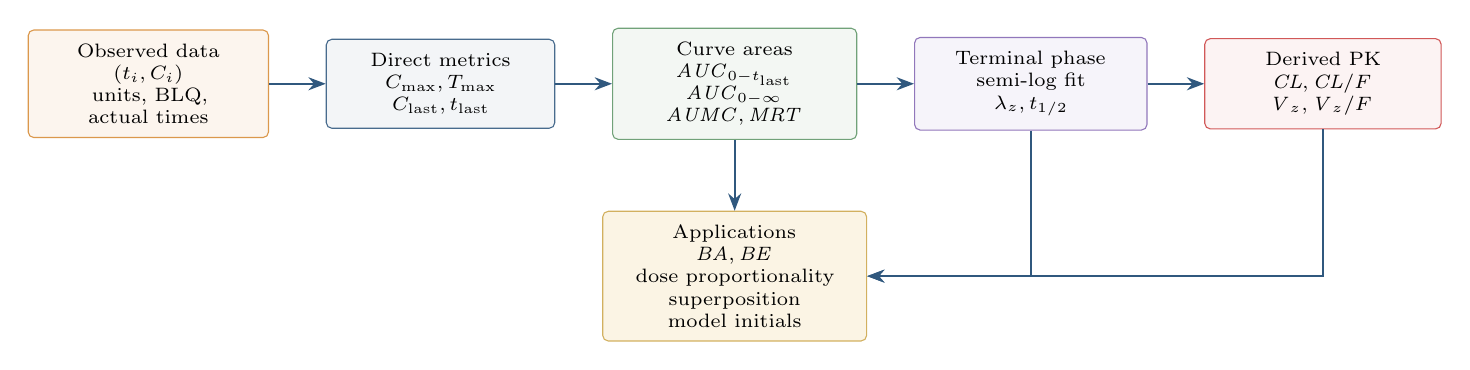
\begin{tikzpicture}[node distance=0.72cm and 0.72cm]
  \node[orangeBox, text width=2.7cm] (data) {Observed data\\ \((t_i,C_i)\)\\ units, BLQ, actual times};
  \node[blueBox, text width=2.55cm, right=of data] (obs) {Direct metrics\\ \(\Cmax,\Tmax\)\\ \(\Clast,\Tlast\)};
  \node[greenBox, text width=2.75cm, right=of obs] (auc) {Curve areas\\ \(\AUClast\)\\ \(\AUCinf\)\\ \(\AUMC,\MRT\)};
  \node[purpleBox, text width=2.6cm, right=of auc] (terminal) {Terminal phase\\ semi-log fit\\ \(\lambdaZ,\halfLife\)};
  \node[redBox, text width=2.65cm, right=of terminal] (derived) {Derived PK\\ \(\CL,\CLF\)\\ \(\Vz,\VzF\)};

  \node[yellowBox, text width=3.0cm, below=0.9cm of auc] (apps) {Applications\\ \(\BA,\BE\)\\ dose proportionality\\ superposition\\ model initials};

  \draw[noteArrow] (data) -- (obs);
  \draw[noteArrow] (obs) -- (auc);
  \draw[noteArrow] (auc) -- (terminal);
  \draw[noteArrow] (terminal) -- (derived);
  \draw[noteArrow] (auc) -- (apps);
  \draw[noteArrow] (derived) |- (apps);
  \draw[noteArrow] (terminal) |- (apps);
\end{tikzpicture}
}
\captionof{figure}{The \NCA{} workflow. The analysis begins with observed concentrations and ends with decision-ready summaries. The terminal slope is not just another metric; it controls extrapolated area, half-life, apparent volume, and non-parametric superposition.}
\end{center}

\subsection{The two hidden assumptions}

The UF lecture names two key assumptions, both about elimination:
\begin{enumerate}[leftmargin=2em]
  \item drug is eliminated only from the central or accessible pool;
  \item terminal decline is mono-exponential.
\end{enumerate}

The first assumption is a statement about where the measured concentration can stand in for the elimination-driving concentration. If liver or kidney clears drug from blood or plasma-accessible drug, a plasma curve is a reasonable summary. If tissue uptake, lysosomal trapping, target-mediated disposition, enterohepatic cycling, long tissue residence, or local tissue metabolism dominates, the plasma tail may be a delayed shadow rather than the actual elimination process. \NCA{} can still be computed, but interpretation becomes more fragile.

The second assumption is the familiar terminal straight line:
\[
  C(t)=C_0 e^{-\lambdaZ t}
  \quad\Longleftrightarrow\quad
  \log C(t)=\log C_0-\lambdaZ t.
\]
The word ``terminal'' is doing real work. We do not require the entire curve to be mono-exponential. Oral absorption can rise, distribution can bend, and multi-compartment movement can create curvature. What \NCA{} needs for \(\AUC_{\Tlast-\infty}\), \(\halfLife\), and \(\Vz\) is a defensible terminal log-linear segment.

\begin{warning}
  \NCA{} is often called ``model independent'', but that phrase should be read gently. Numerical integration of observed data is model-light. Terminal extrapolation is not model-free: it assumes a terminal exponential.
\end{warning}

\section{The Data Object}

\subsection{Observed samples}

The raw material is a subject-level table:
\[
  (t_0,C_0),(t_1,C_1),\ldots,(t_n,C_n),
  \qquad
  0=t_0<t_1<\cdots<t_n.
\]
Here \(t_i\) is time after dose and \(C_i\) is measured concentration in plasma, serum, blood, urine, or another specified matrix. In most plasma \NCA{} work, the table is subject-specific and treatment-period-specific. We compute individual \PK{} parameters first, then summarize them across subjects.

The concentration table is not merely numbers. It carries analysis choices:
\begin{itemize}[leftmargin=2em]
  \item nominal time versus actual sample time;
  \item units, such as \(\pklab{ng/mL}\), \(\pklab{\mu g/L}\), or \(\pklab{mg/L}\);
  \item dose amount and route;
  \item assay lower limit of quantification;
  \item \BLQ{} rules before first measurable concentration and after \Tmax{};
  \item missing samples and protocol deviations;
  \item whether concentration is parent drug, metabolite, total, unbound, or baseline-corrected endogenous compound.
\end{itemize}

The lecture emphasizes ``write a few lines of code or filter in Excel'' for \Cmax{} and \Tmax{}. That is true, but the professional habit is stronger: every derived number should be reproducible from a traceable data table.

\subsection{Direct curve metrics}

Some \NCA{} metrics are read directly from the data:
\[
  \Cmax=\max_i C_i,
  \qquad
  \Tmax=t_j \quad\text{where}\quad C_j=\Cmax.
\]
\[
  \Clast=C_n,
  \qquad
  \Tlast=t_n,
\]
where \(\Clast\) is usually the last measurable or last quantifiable concentration, not necessarily the final scheduled sample if later samples are \BLQ{}.

These four quantities already answer clinically meaningful questions:
\[
\begin{array}{lll}
\Cmax &:& \text{peak systemic concentration;}\\
\Tmax &:& \text{observed time to peak, hence a crude input-rate marker;}\\
\Clast &:& \text{last observed anchor for extrapolation;}\\
\Tlast &:& \text{how far the study followed the curve.}
\end{array}
\]

\Tmax{} deserves special caution. It is an observed order statistic, not a smooth parameter. If sampling is sparse near the peak, \Tmax{} can shift by design rather than biology. In \BE{} work, \AUC{} and \Cmax{} are usually primary because they are more statistically regular; \Tmax{} often remains descriptive unless early onset is clinically important.

\subsection{A small working dataset}

The following toy dataset will be used repeatedly. It is not a fitted model; it is simply a plausible concentration profile after an extravascular dose.

\begin{center}
\resizebox{0.96\textwidth}{!}{%
\begin{tabular}{rrrrrrrrrrr}
\toprule
\(t\) (h) & 0 & 0.5 & 1 & 2 & 4 & 6 & 8 & 12 & 18 & 24\\
\midrule
\(C\) (mg/L) & 0.00 & 1.10 & 2.35 & 3.10 & 2.40 & 1.65 & 1.15 & 0.58 & 0.22 & 0.085\\
\bottomrule
\end{tabular}
}
\captionof{table}{Toy concentration--time data for illustrating \NCA{} calculations.}
\end{center}

From the table:
\[
  \Cmax=3.10\ \pklab{mg/L},
  \quad
  \Tmax=2\ \pklab{h},
  \quad
  \Clast=0.085\ \pklab{mg/L},
  \quad
  \Tlast=24\ \pklab{h}.
\]

\begin{remark}
  In an actual study, the exact same formulas would be applied to each subject. Population means of concentration curves are useful for pictures, but \NCA{} parameter statistics should usually be based on individual parameters, not \NCA{} performed on a mean curve.
\end{remark}

\section{AUC: Exposure as Area}

\subsection{The exact IV bolus derivation}

The cleanest \AUC{} derivation comes from one-compartment \IV{} bolus elimination. Suppose
\[
  C(t)=\frac{D}{V}e^{-(\CL/V)t}.
\]
Then
\[
\begin{aligned}
  \AUCinf
  &=\int_0^\infty C(t)\,\dd t\\
  &=\int_0^\infty \frac{D}{V}e^{-(\CL/V)t}\,\dd t\\
  &=\frac{D}{V}\left[-\frac{V}{\CL}e^{-(\CL/V)t}\right]_0^\infty\\
  &=\frac{D}{V}\cdot\frac{V}{\CL}\\
  &=\frac{D}{\CL}.
\end{aligned}
\]

The beauty is that \(V\) cancels. \AUC{} measures exposure, and for an \IV{} dose under linear elimination, exposure is governed by dose divided by clearance. This is the algebraic reason Module 2 insisted on understanding \CL{} before absorption and \BA{}:
\[
  \CL=\frac{D}{\AUCinf}
  \quad\text{for IV dosing}.
\]

For extravascular dosing, the systemic circulation receives only \(\Fbio D\):
\[
  \AUCinf=\frac{\Fbio D}{\CL},
  \qquad
  \CLF=\frac{D}{\AUCinf}.
\]
The apparent clearance \(\CLF\) is not true clearance unless \(\Fbio\) is known.

\subsection{Why numerical AUC is needed}

In real studies, we do not know the exact continuous function \(C(t)\). We have samples. Therefore \AUC{} is split into two pieces:
\[
  \AUCinf = \AUClast + \pksym{AUC}_{\Tlast-\infty}.
\]
\AUClast{} is estimated by interpolation between observed points. \(\pksym{AUC}_{\Tlast-\infty}\) is extrapolated from \(\Clast\) using the terminal slope.

\begin{center}
\resizebox{0.94\textwidth}{!}{%
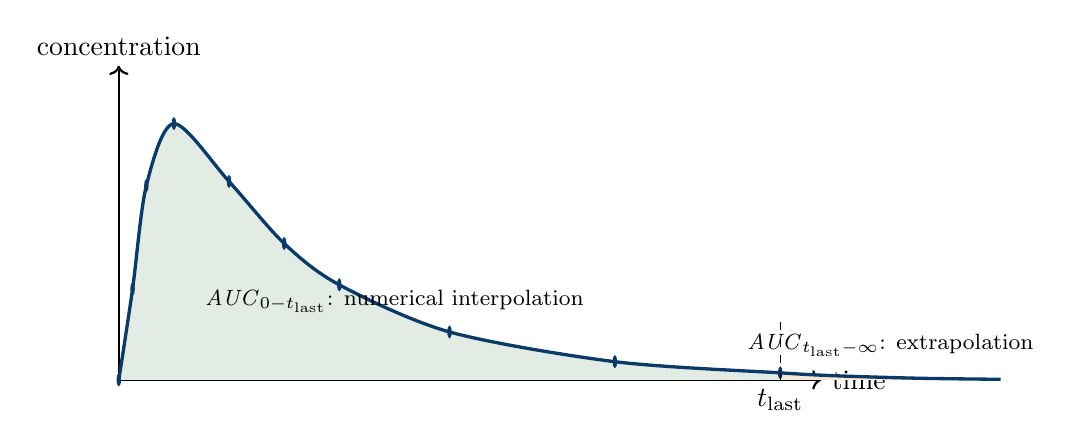
\begin{tikzpicture}[x=0.35cm,y=1.05cm]
  \draw[->, thick] (0,0) -- (25.5,0) node[right]{time};
  \draw[->, thick] (0,0) -- (0,3.8) node[above]{concentration};
  \fill[pkgreen!16] (0,0) -- plot[smooth] coordinates {(0,0) (0.5,1.1) (1,2.35) (2,3.1) (4,2.4) (6,1.65) (8,1.15) (12,0.58) (18,0.22) (24,0.085)} -- (24,0) -- cycle;
  \fill[pkorange!20] (24,0) -- plot[smooth] coordinates {(24,0.085) (26,0.05) (29,0.02) (32,0.007)} -- (32,0) -- cycle;
  \draw[pkblue, very thick] plot[smooth] coordinates {(0,0) (0.5,1.1) (1,2.35) (2,3.1) (4,2.4) (6,1.65) (8,1.15) (12,0.58) (18,0.22) (24,0.085) (26,0.05) (29,0.02) (32,0.007)};
  \foreach \x/\y in {0/0,0.5/1.1,1/2.35,2/3.1,4/2.4,6/1.65,8/1.15,12/0.58,18/0.22,24/0.085}
    \fill[pkblue] (\x,\y) circle (0.08);
  \draw[dashed] (24,0) -- (24,0.7);
  \node[noteLabel] at (10,0.95) {\(\AUClast\): numerical interpolation};
  \node[noteLabel] at (28,0.42) {\(\pksym{AUC}_{\Tlast-\infty}\): extrapolation};
  \node[below] at (24,0) {\(\Tlast\)};
\end{tikzpicture}
}
\captionof{figure}{The two pieces of \AUC{} in \NCA{}. The green part is estimated from observed samples. The orange tail is model-based extrapolation.}
\end{center}

\subsection{Units}

\AUC{} has concentration times time units. If concentration is \(\pklab{mg/L}\) and time is hours, then
\[
  \AUC \quad\text{has units}\quad \pklab{mg\cdot h/L}.
\]
Clearance follows by dimensional cancellation:
\[
  \frac{D}{\AUC}
  =
  \frac{\pklab{mg}}{\pklab{mg\cdot h/L}}
  =
  \pklab{L/h}.
\]
This is a useful self-check. If your \CL{} output has impossible units, the bug is probably in dose units, concentration units, time units, or bioavailability interpretation.

\section{Numerical Integration}

\subsection{Linear trapezoidal method}

For two adjacent samples \((t_1,C_1)\) and \((t_2,C_2)\), the linear trapezoidal area is
\[
  \pksym{AUC}_{t_1-t_2}
  =
  \frac{C_1+C_2}{2}(t_2-t_1).
\]
The derivation is childhood geometry: average of the two parallel sides times width. Equivalently, rectangle plus triangle:
\[
  C_2(t_2-t_1)+\frac{1}{2}(C_1-C_2)(t_2-t_1)
  =
  \frac{C_1+C_2}{2}(t_2-t_1).
\]

Summing over all intervals gives
\[
  \AUClast
  =
  \sum_{i=0}^{n-1}
  \frac{C_i+C_{i+1}}{2}(t_{i+1}-t_i).
\]

\begin{center}
\resizebox{0.82\textwidth}{!}{%
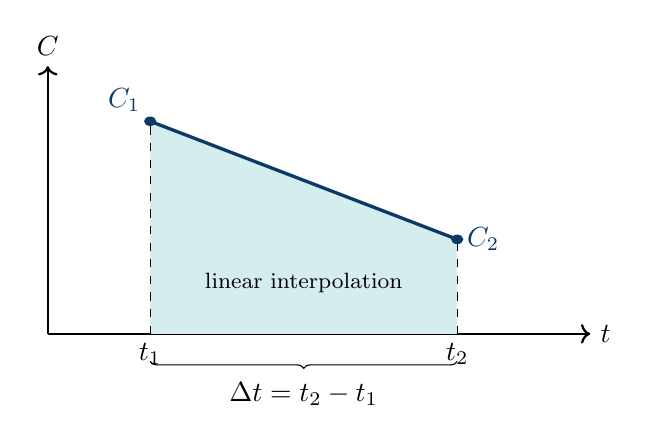
\begin{tikzpicture}[x=1.3cm,y=1.0cm]
  \draw[->, thick] (0,0) -- (5.3,0) node[right]{\(t\)};
  \draw[->, thick] (0,0) -- (0,3.4) node[above]{\(C\)};
  \coordinate (a) at (1,2.7);
  \coordinate (b) at (4,1.2);
  \fill[pkcyan!18] (1,0) -- (a) -- (b) -- (4,0) -- cycle;
  \draw[pkblue, very thick] (a) -- (b);
  \draw[dashed] (1,0) -- (a);
  \draw[dashed] (4,0) -- (b);
  \fill[pkblue] (a) circle (0.06) node[above left]{\(C_1\)};
  \fill[pkblue] (b) circle (0.06) node[right]{\(C_2\)};
  \node[below] at (1,0){\(t_1\)};
  \node[below] at (4,0){\(t_2\)};
  \draw[decorate,decoration={brace,mirror}] (1,-0.35) -- (4,-0.35) node[midway,below=4pt]{\(\Delta t=t_2-t_1\)};
  \node[noteLabel] at (2.5,0.65){linear interpolation};
\end{tikzpicture}
}
\captionof{figure}{Linear trapezoidal area between adjacent observations. It assumes concentration changes linearly between sampled times.}
\end{center}

The method is robust and easy. It performs especially well when sampling is dense or when the curve is close to linear over short intervals. It can overestimate area during exponential decline because the chord lies above a convex decreasing exponential curve.

\subsection{Log trapezoidal method}

If concentration decreases mono-exponentially between \(t_1\) and \(t_2\),
\[
  C(t)=C_1e^{-k(t-t_1)}
  \quad\text{and}\quad
  C_2=C_1e^{-k(t_2-t_1)}.
\]
Solving for \(k\):
\[
  k=\frac{\log C_1-\log C_2}{t_2-t_1}.
\]
The area is
\[
\begin{aligned}
  \pksym{AUC}_{t_1-t_2}
  &=\int_{t_1}^{t_2} C_1e^{-k(t-t_1)}\,\dd t\\
  &=\frac{C_1-C_2}{k}\\
  &=\frac{C_1-C_2}{\log C_1-\log C_2}(t_2-t_1).
\end{aligned}
\]

Thus the log trapezoidal formula is
\[
  \boxed{
  \pksym{AUC}_{t_1-t_2}
  =
  \frac{C_1-C_2}{\log C_1-\log C_2}(t_2-t_1)
  }
  \qquad (C_1>C_2>0).
\]

The assumptions are not cosmetic:
\begin{itemize}[leftmargin=2em]
  \item both concentrations must be positive;
  \item the interval should be decreasing;
  \item exponential interpolation should be scientifically plausible.
\end{itemize}

If \(C_1=C_2\), the limiting value is simply \(C_1(t_2-t_1)\). If either concentration is zero or \BLQ{} treated as zero, log trapezoidal interpolation is undefined.

\subsection{Linear-up log-down}

The practical compromise is \term{linear-up log-down}: use linear trapezoids when concentration rises, and log trapezoids when concentration falls.
\[
\pksym{AUC}_{i,i+1}
=
\begin{cases}
\dfrac{C_i+C_{i+1}}{2}(t_{i+1}-t_i), & C_{i+1}\geq C_i,\\[8pt]
\dfrac{C_i-C_{i+1}}{\log C_i-\log C_{i+1}}(t_{i+1}-t_i), & C_{i+1}<C_i,\ C_i,C_{i+1}>0.
\end{cases}
\]

The logic is pharmacological. During absorption and distribution, the local shape may be complicated and a linear interpolation is a neutral local approximation. During the descending log-linear portion, exponential interpolation respects first-order elimination better.

In software, there are variants: linear trapezoidal, log trapezoidal, linear-up/log-down, and rules that handle repeated rises and falls. The rule should be pre-specified for regulated analyses and reported with the results.

\subsection{Numerical example}

Using the toy dataset, the first interval by linear trapezoid is
\[
  \pksym{AUC}_{0-0.5}
  =
  \frac{0+1.10}{2}(0.5-0)
  =
  0.275\ \pklab{mg\cdot h/L}.
\]
The interval from 2 to 4 hours is decreasing. Linear trapezoidal area is
\[
  \frac{3.10+2.40}{2}(4-2)=5.50.
\]
Log trapezoidal area is
\[
  \frac{3.10-2.40}{\log(3.10)-\log(2.40)}(4-2)
  =
  5.46.
\]
The difference is small here because the interval is short and curvature mild. In sparse terminal sampling, the difference can be larger.

For the full toy table, the linear trapezoidal \(\AUClast\) is approximately
\[
  24.38\ \pklab{mg\cdot h/L}.
\]
The exact value will depend on the selected interpolation rule and any \BLQ{} handling.

\section{Terminal Slope}

\subsection{What lambda z means}

On the terminal log-linear phase,
\[
  C(t)=Ae^{-\lambdaZ t}.
\]
Taking natural logarithms gives
\[
  \log C(t)=\log A-\lambdaZ t.
\]
Therefore, if we fit a line
\[
  y=a+bt,
  \qquad
  y=\log C,
\]
then
\[
  b=-\lambdaZ.
\]
\lambdaZ{} is positive. The fitted terminal slope is negative.

\begin{center}
\resizebox{0.86\textwidth}{!}{%
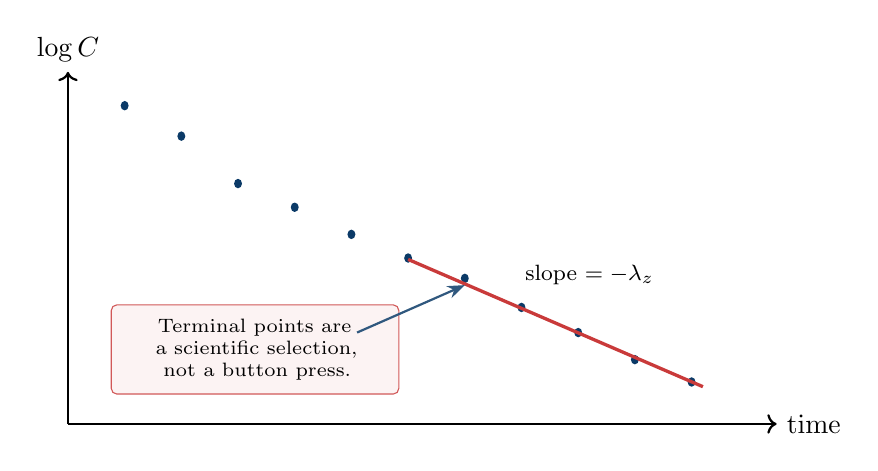
\begin{tikzpicture}[x=0.72cm,y=0.86cm]
  \draw[->, thick] (0,0) -- (12.5,0) node[right]{time};
  \draw[->, thick] (0,0) -- (0,5.2) node[above]{\(\log C\)};
  \foreach \x/\y in {1/4.7,2/4.25,3/3.55,4/3.2,5/2.8,6/2.45,7/2.15,8/1.72,9/1.35,10/0.95,11/0.62}
    \fill[pkblue] (\x,\y) circle (0.07);
  \draw[pkred, very thick] (6,2.43) -- (11.2,0.55);
  \node[redBox, text width=3.3cm] at (3.3,1.1) {Terminal points are a scientific selection, not a button press.};
  \draw[noteArrow] (5.1,1.35) -- (7.0,2.05);
  \node[noteLabel] at (9.2,2.2){slope \(=-\lambda_z\)};
\end{tikzpicture}
}
\captionof{figure}{Terminal slope estimation on a semi-log plot. A visually straight tail supports the exponential extrapolation used by \NCA{}.}
\end{center}

\subsection{Linear regression}

Suppose the selected terminal points are \(j=m,\ldots,n\). Define
\[
  y_j=\log C_j.
\]
The fitted line minimizes residual sum of squares:
\[
  (\hat a,\hat b)
  =
  \argmin_{a,b}
  \sum_{j=m}^{n}(y_j-a-bt_j)^2.
\]
Then
\[
  \hat\lambda_z=-\hat b.
\]

The lecture introduces \(R^2\):
\[
  R^2
  =
  1-\frac{\sum_j(y_j-\hat y_j)^2}{\sum_j(y_j-\bar y)^2}.
\]
A higher \(R^2\) often indicates a straighter terminal segment, but it is not sufficient. Three late points can produce a high \(R^2\) and still represent distribution, flip-flop absorption, assay noise, or a forced fit. Good \NCA{} practice uses residuals, adjusted \(R^2\), span of the terminal phase, number of points, visual inspection, and biological context.

\subsection{Terminal point selection}

Terminal point selection is one of the few places in \NCA{} where judgment is both unavoidable and dangerous. A defensible selection usually asks:
\begin{itemize}[leftmargin=2em]
  \item Are the selected points after absorption and distribution have mostly ended?
  \item Do the selected points form a visually plausible straight line on a semi-log plot?
  \item Does adding an earlier point bend the line?
  \item Does removing a late noisy point change \(\lambdaZ\) materially?
  \item Is the time span long enough to estimate a terminal rate, not just draw a line through adjacent noise?
  \item Is \(\lambdaZ\) consistent with known physiology, earlier studies, or compartmental fits?
\end{itemize}

\begin{warning}
  The last nonzero points are not automatically the terminal phase. For oral drugs with slow absorption, the terminal slope may reflect absorption rate rather than elimination rate. This is the classic flip-flop problem.
\end{warning}

\subsection{Half-life}

Starting from
\[
  C(t)=Ae^{-\lambdaZ t},
\]
\halfLife{} is the time required to reduce concentration by half:
\[
  \frac{A}{2}=Ae^{-\lambdaZ \halfLife}.
\]
Cancel \(A\), take logs, and solve:
\[
  \halfLife=\frac{\log 2}{\lambdaZ}.
\]

The ``five half-lives'' rule follows directly:
\[
  \left(\frac{1}{2}\right)^5=\frac{1}{32}\approx 3.1\%.
\]
After five half-lives, about \(96.9\%\) of a mono-exponentially declining amount has disappeared from that kinetic pool. The same time-scale intuition is used for washout and time to steady state, but only when linear first-order assumptions are reasonable.

\section{Extrapolation to Infinity}

\subsection{The tail formula}

After \Tlast{}, assume
\[
  C(t)=\Clast e^{-\lambdaZ(t-\Tlast)}.
\]
Then
\[
\begin{aligned}
  \pksym{AUC}_{\Tlast-\infty}
  &=\int_{\Tlast}^{\infty}\Clast e^{-\lambdaZ(t-\Tlast)}\,\dd t\\
  &=\frac{\Clast}{\lambdaZ}.
\end{aligned}
\]
Therefore
\[
  \boxed{
  \AUCinf
  =
  \AUClast+\frac{\Clast}{\lambdaZ}
  }.
\]

The extrapolated fraction is
\[
  \%\pksym{AUC}_{\pklab{extra}}
  =
  100\cdot
  \frac{\Clast/\lambdaZ}{\AUCinf}.
\]
Large extrapolated fraction means the total exposure estimate depends heavily on the tail assumption. The UF slide cites an older FDA BA/BE guidance recommending sampling over at least three or more terminal half-lives to capture about 90\% of the relevant \AUC{}. The current FDA 2022 BA guidance continues the same design spirit: adequate sampling is needed to characterize exposure, and the specific design depends on the purpose, dosage form, and study context \cite{fda2022Bioavailability}.

\subsection{AUMC tail and MRT}

For mean residence time we also need the first moment curve:
\[
  \AUMC=\int_0^\infty tC(t)\,\dd t.
\]
The observed part is integrated numerically:
\[
  \AUMClast \approx \sum_i \int_{t_i}^{t_{i+1}} tC(t)\,\dd t,
\]
with formulas depending on the same interpolation choice.

The extrapolated tail has a closed form:
\[
\begin{aligned}
  \pksym{AUMC}_{\Tlast-\infty}
  &=\int_{\Tlast}^{\infty} t\,\Clast e^{-\lambdaZ(t-\Tlast)}\,\dd t\\
  &=\frac{\Tlast\Clast}{\lambdaZ}+\frac{\Clast}{\lambdaZ^2}.
\end{aligned}
\]
Thus
\[
  \AUMCinf
  =
  \AUMClast
  +
  \frac{\Tlast\Clast}{\lambdaZ}
  +
  \frac{\Clast}{\lambdaZ^2}.
\]
Mean residence time is
\[
  \MRT=\frac{\AUMCinf}{\AUCinf}.
\]

\MRT{} is the average time drug molecules spend in the body or sampled kinetic system. For an \IV{} bolus linear system,
\[
  \Vss=\CL\cdot \MRT.
\]
For extravascular data, \(\MRT\) includes input delay. Without additional information, it is not a pure distribution residence time.

\subsection{Worked tail example}

Suppose the toy profile has \(\Clast=0.085\ \pklab{mg/L}\), \(\Tlast=24\ \pklab{h}\), and a terminal fit gives
\[
  \lambdaZ=0.17\ \pklab{h^{-1}}.
\]
Then
\[
  \pksym{AUC}_{24-\infty}
  =
  \frac{0.085}{0.17}
  =
  0.50\ \pklab{mg\cdot h/L}.
\]
If \(\AUClast=24.38\), then
\[
  \AUCinf=24.88,
  \qquad
  \%\pksym{extra}=100\cdot\frac{0.50}{24.88}=2.0\%.
\]
This is a comfortable extrapolated fraction. If instead \(\Clast\) were much higher or \(\lambdaZ\) much smaller, the same sampling schedule might leave a large part of exposure to assumption.

\section{Clearance, Volume, and Residence}

\subsection{Clearance from AUC}

For an \IV{} dose:
\[
  \CL=\frac{D}{\AUCinf}.
\]
For an extravascular dose:
\[
  \CLF=\frac{D}{\AUCinf}.
\]
This is one of the most common interpretation errors in early \PK{} learning. Oral \NCA{} does not identify \(\CL\) and \(F\) separately. A high \(\CLF\) can mean high true clearance, low bioavailability, or both.

The Module 2 lesson should remain in view:
\[
  \AUC_{\PO}=\frac{\Fbio D}{\CL}.
\]
If oral exposure is low, \NCA{} alone cannot tell whether the culprit is dissolution, permeability, gut metabolism, hepatic first pass, or systemic clearance. It can tell us the symptom with precision.

\subsection{Volume from terminal slope}

In a one-compartment terminal relationship,
\[
  \lambdaZ=\frac{\CL}{\Vz}.
\]
Therefore
\[
  \Vz=\frac{\CL}{\lambdaZ}
  \qquad
  \text{or}\qquad
  \VzF=\frac{\CLF}{\lambdaZ}
  \quad\text{after extravascular dosing}.
\]
Substituting \(\CLF=D/\AUCinf\) gives
\[
  \VzF=\frac{D}{\lambdaZ\AUCinf}.
\]

\Vz{} is a terminal-phase apparent volume, not necessarily \Vss{}. It mixes clearance and terminal slope. In multi-compartment systems, a slow terminal slope caused by tissue redistribution can make \Vz{} large even when steady-state distribution has a different meaning.

\subsection{The Rowland-Tozer warning}

Rowland and Tozer's primary-versus-secondary distinction is useful here. \(\halfLife\), \AUC{}, and \(\Vz\) are often derived quantities. They are not always independent mechanistic knobs. For an \IV{} bolus:
\[
  \halfLife=\frac{\log 2}{\lambdaZ},
  \qquad
  \lambdaZ=\frac{\CL}{\Vz}.
\]
So changing \halfLife{} can reflect changing clearance, changing distribution, or both. Similarly, \AUC{} changes can reflect clearance or bioavailability depending on route.

The discipline is to interpret downstream \NCA{} parameters through upstream physiology:
\[
\begin{array}{rcl}
  \AUC &\leftarrow& \CL,\ F,\ \text{dose};\\
  \Cmax,\Tmax &\leftarrow& \text{absorption rate, distribution, clearance, sampling design};\\
  \halfLife &\leftarrow& \CL \text{ and terminal volume};\\
  \Vz &\leftarrow& \CL \text{ and terminal slope};\\
  \MRT &\leftarrow& residence in body plus input delay when extravascular.
\end{array}
\]

\section{Bioavailability and Bioequivalence}

\subsection{Absolute and relative bioavailability}

Absolute bioavailability compares extravascular exposure with intravenous exposure:
\[
  F_{\pklab{abs}}
  =
  \frac{\AUC_{\PO}/D_{\PO}}{\AUC_{\IV}/D_{\IV}}.
\]
If written as a percentage:
\[
  F_{\pklab{abs}}(\%)
  =
  100\cdot
  \frac{\AUC_{\PO}D_{\IV}}{\AUC_{\IV}D_{\PO}}.
\]

Relative bioavailability compares two non-\IV{} products or conditions:
\[
  F_{\pklab{rel}}
  =
  \frac{\AUC_{\pklab{test}}/D_{\pklab{test}}}
       {\AUC_{\pklab{reference}}/D_{\pklab{reference}}}.
\]
This is the natural language for formulation bridging, food effect, route changes, and comparing clinical-trial formulation with the to-be-marketed formulation. FDA's 2022 BA guidance emphasizes that BA data inform safety, effectiveness, dose proportionality, food effect, and formulation life-cycle decisions \cite{fda2022Bioavailability}.

\subsection{Bioequivalence as a statistical statement}

\BE{} is not ``two curves look similar''. It is a statistical claim about rate and extent of absorption, usually based on log-transformed \AUC{} and \Cmax{}.

For most immediate-release systemic products, the modern average \BE{} statement is:
\[
  90\%\ \CI\ \text{for}\ 
  \frac{\text{geometric mean of test}}{\text{geometric mean of reference}}
  \subset [0.8000,1.2500].
\]
FDA's 2001 guidance describes the average \BE{} approach as a 90\% confidence interval for the ratio of population geometric means, usually with 80--125\% limits \cite{fda2001StatisticalBioequivalence}. FDA/ICH M13A 2024 likewise states that, for the majority of drug products, primary \PK{} parameters include \Cmax{} and \(\pksym{AUC}_{0-t}\) in single-dose studies, and their 90\% confidence interval should lie within 80.00--125.00\% \cite{ichM13A2024Bioequivalence}.

\begin{center}
\resizebox{0.90\textwidth}{!}{%
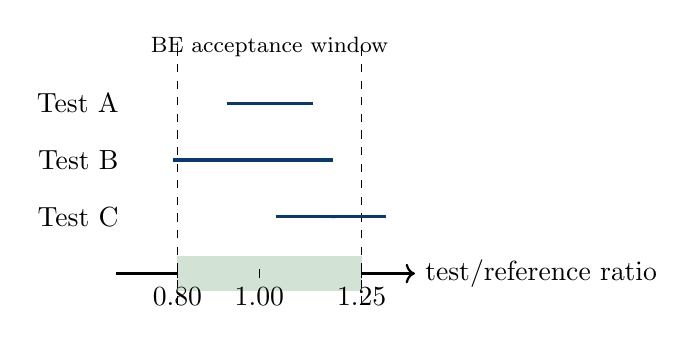
\begin{tikzpicture}[x=5.2cm,y=0.72cm]
  \draw[->, thick] (0.65,0) -- (1.38,0) node[right]{test/reference ratio};
  \draw[pkgreen!25, line width=13pt] (0.80,0) -- (1.25,0);
  \draw[dashed] (0.80,-0.55) -- (0.80,4.1);
  \draw[dashed] (1.25,-0.55) -- (1.25,4.1);
  \foreach \x/\lab in {0.80/0.80,1.00/1.00,1.25/1.25}
    \draw (\x,0.08) -- (\x,-0.08) node[below]{\lab};
  \foreach \y/\name/\lo/\mid/\hi in {3/Test A/0.92/1.02/1.13,2/Test B/0.79/0.98/1.18,1/Test C/1.04/1.18/1.31}
  {
    \draw[pkblue, very thick] (\lo,\y) -- (\hi,\y);
    \fill[pkblue] (\mid,\y) circle (0.022);
    \node[left] at (0.68,\y){\name};
  }
  \node[noteLabel] at (1.025,4.0){BE acceptance window};
\end{tikzpicture}
}
\captionof{figure}{A schematic \BE{} plot. Test A passes because the full 90\% CI lies in 0.80--1.25. Test B and Test C fail because one confidence bound crosses the window, even if the point estimate looks close.}
\end{center}

The metoprolol extended-release case discussed in the UF slide deck illustrates why \NCA{} metrics matter in formulation evaluation: release-rate changes can leave one metric acceptable while another exposes a clinically relevant difference \cite{kim2019MetoprololFormulation}. For modified-release products, shape, partial \AUC{}, and dosing interval behavior may matter beyond total \AUC{} and \Cmax{}.

\subsection{M13A updates}

\ICH{} M13A is important because it harmonizes scientific and technical expectations for \BE{} studies of orally administered immediate-release solid oral dosage forms. Three points are especially relevant for Module 3:
\begin{itemize}[leftmargin=2em]
  \item \textbf{Primary parameters.} For most single-dose \BE{} studies, \(\pksym{AUC}_{0-t}\) and \Cmax{} are the core parameters. \(\AUCinf\), \(\Tmax\), \(\lambdaZ\), and \(\halfLife\) are additional descriptors.
  \item \textbf{Sampling.} The sampling schedule should capture the concentration--time profile sufficiently for \AUC{} and \Cmax{}, with special consideration for early exposure, long half-life drugs, and partial \AUC{} when onset matters.
  \item \textbf{Data presentation.} Individual and mean concentration--time plots on linear and log-linear scales should be provided, and concentration data should be tabulated with deviations identified.
\end{itemize}

This means \NCA{} is not a side calculation at the end of a study. It influences study design before the first subject is dosed.

\section{Dose Proportionality and Linearity}

\subsection{What dose proportionality asks}

If \PK{} is linear and bioavailability does not change with dose, then
\[
  \AUC \propto D,
  \qquad
  \Cmax \propto D.
\]
Equivalently, dose-normalized exposure is constant:
\[
  \frac{\AUC}{D}\approx\text{constant},
  \qquad
  \frac{\Cmax}{D}\approx\text{constant}.
\]

NCA metrics are therefore the natural response variables for dose proportionality. A common model is the power model:
\[
  \log Y = \alpha+\beta\log D+\epsilon,
\]
where \(Y\) might be \AUC{} or \Cmax{}. Perfect dose proportionality corresponds to
\[
  \beta=1.
\]

\subsection{How nonlinearity appears}

Nonlinearity can enter through any Module 2 mechanism:
\begin{itemize}[leftmargin=2em]
  \item saturable absorption or dissolution limits;
  \item saturable gut or hepatic first-pass metabolism;
  \item saturable renal secretion;
  \item concentration-dependent protein binding;
  \item target-mediated drug disposition;
  \item solubility-limited exposure at high doses;
  \item time-varying induction or inhibition.
\end{itemize}

NCA detects the footprint before it explains the mechanism. If \AUC{} rises more than proportionally with dose, clearance may be decreasing, first pass may be saturating, or bioavailability may be increasing. If \Cmax{} rises less than proportionally while \AUC{} remains proportional, absorption rate or formulation dissolution may be changing more than extent.

\subsection{A useful diagnostic table}

\begin{center}
{\footnotesize
\begin{tabularx}{0.96\textwidth}{p{0.21\textwidth}p{0.14\textwidth}p{0.15\textwidth}X}
\toprule
Observation & \AUC{} & \Cmax{} & First interpretation\\
\midrule
Proportional & \(\uparrow\) with dose & \(\uparrow\) with dose & Linear exposure over tested range.\\
More than proportional \AUC{} & high & high or mixed & Saturable clearance or increasing \(F\).\\
Less than proportional \AUC{} & low & low & Solubility, absorption, degradation, or reduced \(F\).\\
\Cmax{} changes more & similar extent & altered peak & Rate/formulation/input-rate effect.\\
\Tmax{} shifts & similar extent & peak timing changes & Absorption timing, food, gastric emptying, release profile.\\
\bottomrule
\end{tabularx}
}
\captionof{table}{NCA metrics as a first diagnostic for dose proportionality and formulation effects.}
\end{center}

\section{Non-Parametric Superposition}

\subsection{The idea}

Non-parametric superposition predicts multiple-dose or steady-state concentrations from a single-dose profile without fitting a compartmental model. The idea is linear systems thinking:
\[
  \text{multiple-dose curve}
  =
  \text{sum of shifted single-dose curves}.
\]
If the dosing interval is \(\tau\), then a simple superposition expression is
\[
  C_{\pklab{ss}}(t)
  =
  \sum_{k=0}^{\infty} C_{\pklab{single}}(t+k\tau),
  \qquad
  0\leq t<\tau,
\]
where the unobserved late tail is extended using \(\lambdaZ\).

For a pure terminal exponential, the accumulation ratio is
\[
  R=\frac{1}{1-e^{-\lambdaZ\tau}}.
\]
This is the same geometric-series logic behind repeated first-order dosing.

\subsection{Assumptions}

The UF lecture states the core assumptions:
\begin{itemize}[leftmargin=2em]
  \item each dose acts independently of every other dose;
  \item rate and extent of absorption are the same for each dosing interval;
  \item average systemic clearance is the same for each dosing interval;
  \item linear \PK{} applies, meaning dose proportionality and time-invariant kinetics.
\end{itemize}

These assumptions exclude many real complications: autoinduction, time-dependent inhibition, saturable absorption, adherence variation, disease evolution, target-mediated clearance, formulation changes across doses, and circadian biology. But when the assumptions are reasonable, superposition is a beautiful bridge from single-dose \NCA{} to steady-state prediction.

\subsection{Visualization}

\begin{center}
\resizebox{0.92\textwidth}{!}{%
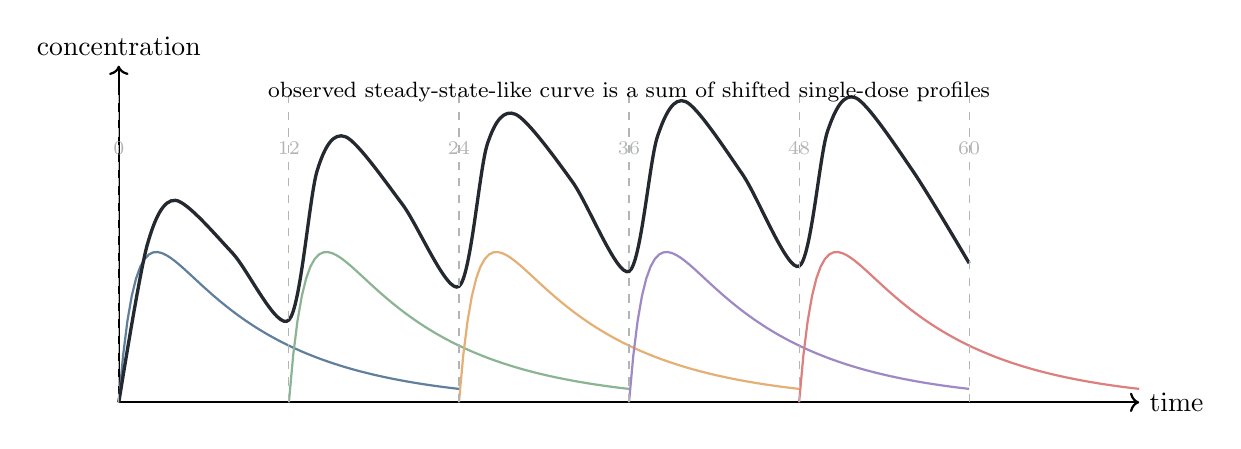
\begin{tikzpicture}[x=0.18cm,y=0.95cm]
  \draw[->, thick] (0,0) -- (72,0) node[right]{time};
  \draw[->, thick] (0,0) -- (0,4.5) node[above]{concentration};
  \foreach \shift/\col in {0/pkblue,12/pkgreen,24/pkorange,36/pkpurple,48/pkred}
  {
    \draw[\col!65, thick, domain=0:24, samples=80, variable=\x]
      plot ({\x+\shift},{3.2*(1-exp(-0.75*\x))*exp(-0.12*\x)});
  }
  \draw[pkink, very thick] plot[smooth] coordinates {
    (0,0.0) (2,2.1) (4,2.7) (8,2.0) (12,1.1)
    (14,3.1) (16,3.55) (20,2.65) (24,1.55)
    (26,3.45) (28,3.85) (32,2.95) (36,1.75)
    (38,3.55) (40,4.02) (44,3.05) (48,1.82)
    (50,3.62) (52,4.07) (56,3.10) (60,1.86)
  };
  \foreach \x in {0,12,24,36,48,60}
    \draw[dashed, pkink!35] (\x,0) -- (\x,4.2) node[below=16pt, font=\scriptsize]{\(\x\)};
  \node[noteLabel] at (36,4.15){observed steady-state-like curve is a sum of shifted single-dose profiles};
\end{tikzpicture}
}
\captionof{figure}{Schematic non-parametric superposition. Individual shifted single-dose contributions accumulate into a multiple-dose concentration curve.}
\end{center}

\section{Hands-On NCA Workflow}

\subsection{Before running software}

Before pressing ``run'', decide what the analysis means.
\begin{enumerate}[leftmargin=2em]
  \item Identify route, dose, dosing time, matrix, analyte, units, and subject-period structure.
  \item Decide whether actual times or nominal times are used.
  \item Define \BLQ{} handling before first quantifiable sample, between quantifiable samples, and after \Tmax{}.
  \item Choose the interpolation rule: linear, log, or linear-up/log-down.
  \item Pre-specify terminal slope selection rules or at least document manual selection rationale.
  \item Decide which parameters are primary, secondary, and exploratory.
  \item Check whether extravascular parameters should be reported as apparent values: \(\CLF\), \(\VzF\).
\end{enumerate}

This is where \NCA{} resembles statistics more than arithmetic. The formulas are simple. The analysis plan protects the formulas from becoming arbitrary.

\subsection{After running software}

After software output, do not go straight to the parameter table. Inspect:
\begin{itemize}[leftmargin=2em]
  \item individual linear-scale concentration--time plots;
  \item individual semi-log plots with selected terminal points;
  \item \(\lambdaZ\) fit statistics and residuals;
  \item \(\%\AUC_{\pklab{extra}}\);
  \item units and dose normalization;
  \item impossible values such as negative half-life, \(\AUCinf<\AUClast\), or enormous apparent volume from a poor terminal slope;
  \item subject profiles with vomiting, missed samples, protocol deviations, or suspicious \BLQ{} patterns.
\end{itemize}

For \BE{} or \BA{} studies, the individual curve plots are not decoration. Current FDA/ICH expectations emphasize tabulated concentration data and both individual and mean plots on linear and log-linear scales \cite{ichM13A2024Bioequivalence}.

\subsection{A reproducibility checklist}

\begin{center}
\begin{tabularx}{0.96\textwidth}{lX}
\toprule
Item & What should be recorded\\
\midrule
Study context & Route, formulation, dose, fasted/fed, single/multiple dose, analyte.\\
Data handling & Actual/nominal time, missing values, \BLQ{} rule, baseline correction if endogenous.\\
AUC method & Linear, log, linear-up/log-down, partial \AUC{} windows.\\
Terminal slope & Points selected, fit method, \(R^2\), adjusted \(R^2\), time span, exclusions.\\
Derived parameters & Whether \(\CL\) or \(\CLF\), \(\Vz\) or \(\VzF\), \(\Vss\) only when justified.\\
Regulatory comparison & Log transform, \GMR{}, 90\% \CI{}, acceptance window, primary metrics.\\
\bottomrule
\end{tabularx}
\captionof{table}{Minimum reproducibility metadata for a serious \NCA{} result.}
\end{center}

\section{What NCA Can and Cannot Tell You}

\subsection{What NCA is excellent at}

\NCA{} is excellent when the question is:
\begin{itemize}[leftmargin=2em]
  \item What was systemic exposure?
  \item How high was the peak concentration?
  \item When did the observed peak occur?
  \item What is the apparent terminal half-life?
  \item What is apparent clearance or apparent volume after this route?
  \item Are two formulations similar in rate and extent of absorption?
  \item Is exposure dose proportional over the tested range?
  \item What initial parameter guesses might help a compartmental model?
\end{itemize}

These are not minor questions. Many label, formulation, and clinical pharmacology decisions can be made from these summaries when the study is designed well.

\subsection{Where NCA becomes fragile}

\NCA{} becomes fragile when the question requires hidden mechanisms:
\begin{itemize}[leftmargin=2em]
  \item separating absorption from elimination in flip-flop kinetics;
  \item identifying tissue compartments;
  \item estimating target-site concentration;
  \item extrapolating outside observed dose, route, formulation, or population;
  \item predicting untested regimens under nonlinearity;
  \item distinguishing low \(F\) from high \CL{} after oral dosing;
  \item modeling time-varying clearance, induction, inhibition, or disease progression;
  \item connecting exposure to response with delays, tolerance, turnover, or feedback.
\end{itemize}

That is where compartmental \PK{}, \PKPD{}, population modeling, physiologically based \PK{}, and Bayesian inference enter. \NCA{} summarizes the curve; mechanistic models explain and predict the curve.

\subsection{The DiStefano distinction}

DiStefano's classic discussion of noncompartmental versus compartmental analysis is still useful because it prevents a false rivalry \cite{distefano1982Noncompartmental}. The choice is not ``simple versus real''. It is question-dependent:
\begin{center}
\begin{tabularx}{0.92\textwidth}{lX}
\toprule
\NCA{} & minimal structural assumptions, direct empirical summaries\\
Compartmental model & explicit structure, latent states, simulation, extrapolation\\
\bottomrule
\end{tabularx}
\end{center}
The right workflow often uses both. Run \NCA{} first to understand observed exposure, half-life, and plausible starting values. Then fit a compartmental model if the scientific question demands mechanism, prediction, covariates, sparse data borrowing, or simulation.

\section{Summary}

\subsection{One paragraph}

Module 3 turns a concentration--time table into decision-ready pharmacokinetics. \Cmax{}, \Tmax{}, \Clast{}, and \Tlast{} are read directly from observed data. \AUClast{} is numerical geometry, usually linear or linear-up/log-down trapezoidal interpolation. \AUCinf{} adds a terminal exponential tail \(\Clast/\lambdaZ\), which makes terminal slope selection one of the key scientific judgments in \NCA{}. The same terminal slope gives \(\halfLife=\log 2/\lambdaZ\), while \AUC{} gives \(\CL=D/\AUC\) for \IV{} dosing and \(\CLF=D/\AUC\) for extravascular dosing. \(\Vz=\CL/\lambdaZ\), \(\Vss=\CL\cdot\MRT\) for appropriate \IV{} settings, and \(\MRT=\AUMC/\AUC\) connect exposure to residence. These metrics support \BA{}, \BE{}, dose proportionality, non-parametric superposition, and starting values for compartmental models. The central discipline is interpretation: \NCA{} is empirical curve geometry plus terminal exponential assumptions, not a full mechanism of absorption, distribution, metabolism, and excretion.

\subsection{Formula sheet}

\[
  \Cmax=\max_i C_i,
  \qquad
  \Tmax=t_i \text{ at } \Cmax,
  \qquad
  \Clast=C_n,
  \qquad
  \Tlast=t_n.
\]
\[
  \pksym{AUC}_{t_i-t_{i+1}}^{\pklab{linear}}
  =
  \frac{C_i+C_{i+1}}{2}(t_{i+1}-t_i).
\]
\[
\begin{aligned}
  \pksym{AUC}_{t_i-t_{i+1}}^{\pklab{log}}
  &=
  \frac{C_i-C_{i+1}}{\log C_i-\log C_{i+1}}(t_{i+1}-t_i),\\
  &\hspace{2.2cm} C_i>C_{i+1}>0.
\end{aligned}
\]
\[
  \AUCinf=\AUClast+\frac{\Clast}{\lambdaZ},
  \qquad
  \%\pksym{extra}=100\cdot\frac{\Clast/\lambdaZ}{\AUCinf}.
\]
\[
\begin{aligned}
  \halfLife&=\frac{\log 2}{\lambdaZ},\\
  \CL&=\frac{D}{\AUCinf}\quad \text{for IV},\\
  \CLF&=\frac{D}{\AUCinf}\quad \text{for extravascular}.
\end{aligned}
\]
\[
  \Vz=\frac{\CL}{\lambdaZ},
  \qquad
  \VzF=\frac{\CLF}{\lambdaZ}.
\]
\[
  \AUMCinf
  =
  \AUMClast
  +
  \frac{\Tlast\Clast}{\lambdaZ}
  +
  \frac{\Clast}{\lambdaZ^2},
  \qquad
  \MRT=\frac{\AUMCinf}{\AUCinf}.
\]
\[
\begin{aligned}
  F_{\pklab{abs}}
  &=
  \frac{\AUC_{\PO}/D_{\PO}}{\AUC_{\IV}/D_{\IV}},\\
  F_{\pklab{rel}}
  &=
  \frac{\AUC_{\pklab{test}}/D_{\pklab{test}}}
       {\AUC_{\pklab{reference}}/D_{\pklab{reference}}}.
\end{aligned}
\]
\[
\begin{aligned}
  \BE:\quad
  90\%\ \CI\{\GMR_{\pklab{test/reference}}\}
  &\subset [0.80,1.25]\\
  &\text{for most average BE settings.}
\end{aligned}
\]

\subsection{Questions I should be able to answer}

\begin{itemize}[leftmargin=2em]
  \item Why is \AUC{} equal to \(D/\CL\) after \IV{} bolus dosing under linear elimination?
  \item Which part of \AUC{} is numerical interpolation and which part is model-based extrapolation?
  \item When should log trapezoidal interpolation be preferred over linear trapezoidal interpolation?
  \item Why is terminal slope selection not a purely automatic problem?
  \item Why can oral \NCA{} estimate \(\CLF\) but not \CL{} alone?
  \item Why are \Cmax{} and \Tmax{} rate-related but not pure absorption parameters?
  \item What does \(\%\pksym{AUC}_{\pklab{extra}}\) warn us about?
  \item Why does \BE{} use geometric mean ratios and 90\% confidence intervals?
  \item What assumptions make non-parametric superposition reasonable?
  \item When should I stop using \NCA{} alone and move to a compartmental or population model?
\end{itemize}

\bibliographystyle{plain}
\bibliography{../refs/pharmacology}

\end{document}
